\problemname{Driving Lanes}

While driving around a curve on the highway, Sam realizes that if they
use the inside lane, they travel a shorter distance. Sam wonders what
is the minimum distance needed to travel to the destination.
%across the entire highway.



The multilane highway consists of a sequence of straightaways that are
connected by curves. When going around a curve, the distance travelled
depends on which lane you are in. Each curve has a curvature $c$ and
stretch $s$. Specifically, if Sam is in lane $i$, then they travel
$s + c \cdot i$ meters while going around this curve.



Whenever Sam is on a straightaway, they may change from one lane into
an adjacent lane.  When changing to an adjacent lane, Sam moves
forward $k$ meters, but travels a total of $k+r$ meters.  Each lane
change must be completed before the car reaches the end of the current
straightaway.  Sam may change lanes multiple times in the same
straightaway. For safety reasons, changing lanes is not possible on
curves.

\begin{center}
 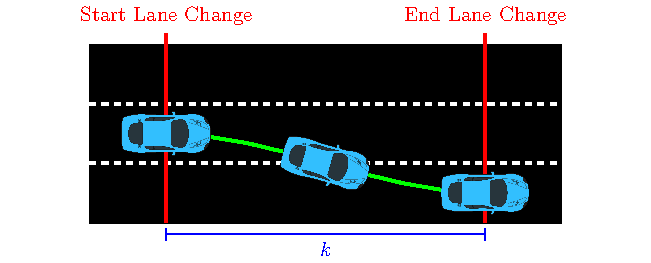
\includegraphics[width=0.8\textwidth]{chla.pdf}
\end{center}

Sam starts in lane $1$ and wishes to end in lane $1$. What is the minimum
distance they must travel?



\section*{Input}

The first line of input contains two integers
$n$~($1 \leq n \leq 250$), which is the number of straightaways, and
$m$~($1 \leq m \leq 250$), which is the number of lanes on the
highway. The lanes are numbered $1, 2, \dots, m$.



The second line of input contains two integers
$k$~($1 \leq k \leq 10^6$) and $r$~($1 \leq r \leq 10^6$), which are
the lane changing parameters.



The next $n$ lines describe the straightaways in order. Each of these lines
contains a single integer $\ell$~($1 \leq \ell \leq 10^6$), which is
the length of this straightaway.



The next $n-1$ lines describe the curves in order. Each of these lines contains
two integers $s$~($1 \leq s \leq 10^6$), which is the stretch of
this curve, and $c$~($-10^6 \leq c \leq 10^6$), which is the curvature of
this curve. It is guaranteed that $s + c \cdot m > 0$.

The $i$th curve connects the $i$th and $(i+1)$th straightaway.



\section*{Output}

Display the minimum distance Sam must travel.
